\section{American Fuzzy Lopper (AFL)} 
\label{sec:2-afl}

Michal Zalewski developed American Fuzzy Lopper as a coverage-guided greybox fuzzer. He introduces this open-source project as \say{a security-oriented fuzzer that employs a novel type of compile-time instrumentation and genetic algorithms to automatically discover clean, interesting test inputs that trigger new internal states of the targeted binary. This substantially improves the functional coverage for the fuzzed code. The compact synthesized corpus produced by the tool help seed other, more labor- or resource-intensive testing regimes down the road.} \cite{zalewski2014american} AFL is designed to perform \textbf{fast} and \textbf{reliable}, and at the same time, benefits from the \textbf{simplicity} and \textbf{chainability} features \cite{about_afl}:

\begin{itemize}
    \item \textbf{Speed:} Avoiding the time-consuming operations and increasing the number of executions over time.
    \item \textbf{Reliability:} AFL takes strategies that are program-agnostic, leveraging only the coverage metrics for more discoveries. This feature helps the fuzzer to perform consistently in finding the vulnerabilities in different programs.
    \item \textbf{Simplicity:} AFL provides different options, helping the users enhance the fuzz testing in a straightforward and meaningful way. 
    \item \textbf{Chainability:} AFL can test any binary which is executable and is not constrained by the target software. A driver for the target program can connect the binary to the fuzzer. 
\end{itemize}

\begin{figure}[!b]
    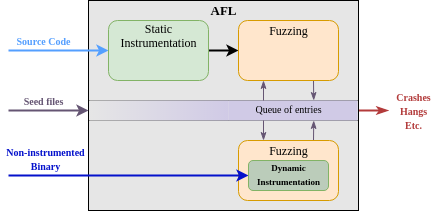
\includegraphics[width=\textwidth]{Chapter2/AFL-io.png}
    \centering
    \captionsetup{justification=centering}
    \caption{AFL's procedure: simplified}
    \label{fig:afl-io}
\end{figure}

% The simplified version of the AFL
AFL tests the program by running the program and monitoring the execution path for each run. To extract information from a run, AFL offers multiple \textbf{instrumentation} techniques for constructing hashes of the explored paths while following the executing path of the actual program. AFL requires instrumented binaries which provide the execution information when they are run by AFL. AFL is a whitebox/greybox fuzzer when it can effectively insert the instrumentations into the program. Figure \ref{fig:afl-io} shows a simplified illustration of the procedure of AFL. In whitebox fuzzing, AFL takes the source code of the program and executes static instrumentation during the compilation of the program, and passes the generated binary to the fuzzing module. On the other hand, the greybox feature of AFL lets the fuzzer to execute the un-instrumented binary under a dynamic instrumentation, which executes the instrumenting instructions wrapped around the basic blocks of the program.

% Instrumentation features - Coverage calculations.

\subsection{Instrumentation}
\label{subsec:instrumentation}

The collection of coverage information is generated during the execution; when the execution steps into a basicblock, the procedure \ref{lst:hash} stores the visited edge (pair of two consecutive basicblocks) in CFG. The hashing only stores the information from the previous basicblock and the current basicblock which we are already in. For instance, suppose we have CFG of a program as shown in \ref{fig:instrumentation}; by giving the persmission to the program to modify a memory region shared with AFL - which AFL also has access to it - the coverage instructions generate a summary of the executed path. For example, suppose we have an instrumented program with the random values which are set in compile time (for simplicity, suppose that initially random value $cur\_location=1010$). Running the first basic block assigns $CUR\_HASH$ to $73\oplus1010=955$; the content of index $955$ of shared memory is then increased by one, and the execution continues to the next basic block. If the execution is jumped into basicblock 2, the content of $shared\_mem[310\oplus(73>>1)=274]$ is incremented by one, and so on. This procedure continues along with the main execution and in the end, the content of the shared memory contains a hashing of the traveled path. In this scenario, taking the path $1\rightarrow2\rightarrow5$ results in an array of zeros except for $\{51: 1, 274: 1, 955: 1\}$ as the hashed path.

\begin{lstlisting}[language=C++,style=CodeStyle,label={lst:hash},caption={Select element and update in shared\_mem}]
    cur_location = <COMPILE_TIME_RANDOM>;
    shared_mem[cur_location ^ prev_location]++; 
    prev_location = cur_location >> 1;
\end{lstlisting}

\begin{figure}[htpb]
    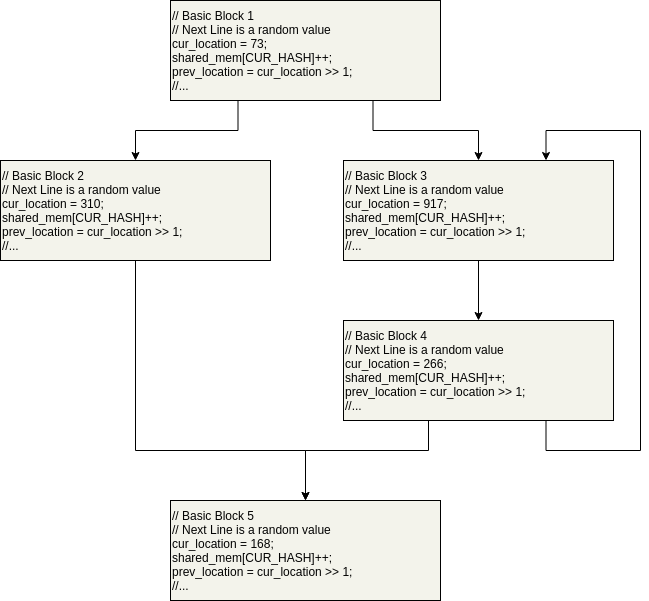
\includegraphics[width=\textwidth]{Chapter2/instrumentation.png}
    \centering
    \captionsetup{justification=centering}
    \caption{Example for instrumented basic blocks}
    \label{fig:instrumentation}
\end{figure}

AFL uses both dynamic and static instrumentation for profiling executions. Static instrumentation is applied using \textbf{LLVM} modules which can analyze and insert instructions anywhere in the program. Dynamic instrumentation is another method which let let the fuzzer to use the instrumentation instructions while executing the program. By default, AFL uses \texttt{QEMU} for dynamic instrumentation \cite{afl_qemu}. The emulator wraps the genuine instructions into analyzable modules, and constructs the execution path while running. This technique, \textbf{qemu-mode}, causes a slow down of 10-100\% for each execution compared to the \textbf{llvm-mode}. For the purpose of this article, we need to dig more into the procedure of instrumentation in llvm-mode \cite{afl-llvm}.

\subsubsection{LLVM}
\label{subsub:llvm}

\begin{figure}[!b]
    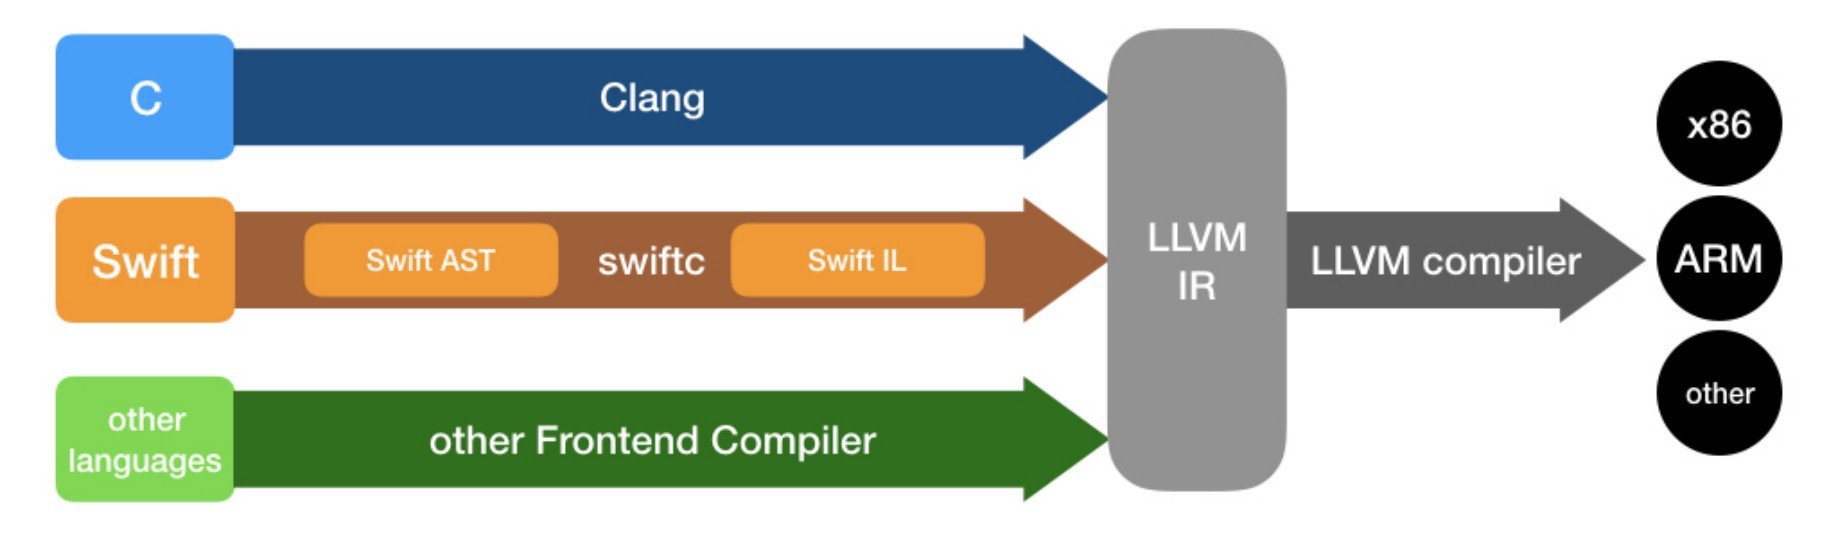
\includegraphics[width=\textwidth]{Chapter2/llvm.png}
    \centering
    \captionsetup{justification=centering}
    \caption{LLVM architecture: A front-end compiler generates the LLVM IR, and then it is converted into machine code \cite{omni_sci}}
    \label{fig:llvm}
\end{figure}

\say{The LLVM Project is a collection of modular and reusable compiler and toolchain technologies. Despite its name, LLVM has little to do with traditional virtual machines. The name \textbf{LLVM} itself is not an acronym; it is the full name of the project.} \cite{llvm} Two of the relevant projects used by AFL are:

\begin{itemize}
    \item The \textbf{LLVM Core} libraries contain source/target-independent optimizers as well as code generators for popular CPUs. These well-documented modules assist development of a custom compiler in every step (\textit{pass}) through the conversion of source code to executable binary file.
    
    \item \textbf{Clang} \cite{clang} provides a front-end for compiling C language family (C, C++, Objective C/C++, OpenCL, CUDA, and RenderScript) for the LLVM Project. Clang uses the LLVM Core libraries to generate an \textit{Intermediate Representation} (\textbf{IR}) of the source code \cite{lattner2004llvm}. The IR is then translated into an executable binary for the machine's CPU (Figure \ref{fig:llvm}).
\end{itemize}

AFL utilizes the compilation \textit{passes} of Clang with a custom recipe for \textit{module pass}. Passes are the modules performing the transformations and optimizations of a compilation. Each pass is applied on a specified section of the code. For instance, the \textbf{ModulePass} class (and any classes derived from this class) performs the analysis of the code and the insertion of new instructions. Other classes such as \textbf{FunctionPass}, \textbf{LoopPass}, and etc perform their instructions using different parts of the code, and they contain less information about the rest of the program. AFL uses only the ModulePass and iterates over every basicblock existing in the program

\subsection{AFL Fuzz}

% Start of the fuzz testing
The automatic fashion of testing a targeted software using AFL requires a modified execution of the software with coverage-based instructions. The coverage-based instructions are used during the fuzz testing to provide a summary of the execution under AFL's supervision. AFL passes the next test case from the queue of entries to the program, and \textit{caliberates} the test case so that it is ready to be fuzzed. After the calibration of the case, AFL tries to trim the case such that the execution's profile remains the same.

% How it is continued
AFL fuzzes the case after it's preperations; different mutation techniques are applied to the test case, and the newly generated test cases are analyzed to check if they are producing any new execution behavior based on their code coverage and execution's $speed \times file\_size$. The cases which pass the prior check are considered as \textit{interesting} cases and are added to the queue of entries. We will investigate the details of this functionality later in this article. 

% Fuzzing techniques
AFL uses various mutation techniques for fuzzing a case. There are two main stages for mutations:
\begin{itemize}
    \item \textbf{Deterministic} stage: This early stage contains a sequence of operations which contain:
    \begin{enumerate}
        \item Sequential bit flips with varying lengths and stepovers
        \item Sequential additions and subtractions of small integers
        \item Sequential insertion of know interesting integers - such as \textit{0}, \textit{1}, \texttt{\textit{MAX\_INT}} and etc. \cite{about_afl}
        \item Sequential replacement of content of the case by dictionary tokens provided: AFL accepts a dictionary of known values - such as magic values used in the header of a file. For instance, a dictionary for HTML tags which is also provided in the AFL's repository, contains known HTML patterns such as \texttt{tag\_header="<header>"
        }, which AFL would use to replace some bytes of the content of the case with string \texttt{<header>}.
    \end{enumerate}
    
    \item \textbf{Non-deterministic} stage: This stage contains two main operations:
    \begin{enumerate}
        % TODO: Describe perf score as it is an important feature that may interfere with our work
        \item Random HAVOC: A sequence of random mutations are applied on the input in this stage. The operations include actions on file such as insertion and deletion of random bytes, cloning subsequences of input, and etc. The repetition of this stage depends on the \textbf{performance score} of the current case under investigation. AFL calculates this score based on the code coverage of the test case and it's execution speed; the more locations visited stored in \textit{coverage bitmap}, and the lower the execution speed are prefereable, and as a result, AFL increases the score based on that. 
        \item Splicing: If non of the previous stages result in any new findings, AFL tries selecting a random case from the queue, and copies a subsequence of that case into the current case, and relies on the HAVOC stage for mutating the results.
    \end{enumerate}
\end{itemize}

% Update bitmap score
As we discussed, the input files generated for the target program after the fuzzing phase are processed for any \textit{interesting} feature. This procedure goes through two functions called as \texttt{save\_if\_interesting()} and \textit{update\_bitmap\_score()}:

\begin{itemize}
    \item \textbf{\texttt{save\_if\_interesting()}}: This function checks if there are any new bits in the shared trace bits (which stores the coverage information) and if a finding is showing new previously unset bits, it tags the case as an interesting one. This function also summerizes the trace bits to reduce the processing effort in later checks - to compare new findings with this generated case.

% Save if interesting
    \item \textbf{\texttt{update\_bitmap\_score()}}: AFL maintains a list of \texttt{top\_rated[]} entries for every byte in the bitmap. Each element of the \texttt{top\_rated[]} entries tracks the fastest \texttt{queue\_entry} which visits an edge.
\end{itemize}

% Cull queue
AFL analyzes the cases using the above provided functions, and the best queue entries are updated eventually in the fuzzing procedure. To select the next element of the queue for fuzzing, AFL uses this information for tagging the \textit{favorite} and \textit{redundant} entries. These operations are done under the function \textit{cull\_queue()}. Each element of the list \texttt{top\_rated[]} contains a pointer to the \texttt{queue\_entries[]}, and marks the pointed entry as a \texttt{favored} entry. After a complete walk over the list, the remaining unfavored entries are marked as \texttt{redundant}. In every fuzzing cycle over the queue entries, \texttt{cull\_queue()} prepares the queue and then AFL takes the next front entry which is also \textit{favored}.

% MAYBE: explain the structure of top_rated[] entries

% AFL's static instrumentation starts with the allocation of a shared memory. This shared memory stands between AFL's fuzzer and each program's execution. Everytime the instrumentated program is run, the injected instructions fill the shared memory with the coverage status of the execution. After the termination of the process, AFL continues its fuzzing procedure. Shared memory is updated with new execution's data, and AFL can use it to evaluate the performance of the recent execution. The runtime initialization recipe is saved in \texttt{llvm-mode/waffle-llvm-rt.o.c} of the project.

% An snippet of the AFL's instrumentation pass is shown in Listing \ref{lst:afl-llvm}.

% \lstinputlisting[language=C++,style=CodeStyle,label={lst:afl-llvm},caption={AFLCoverage module}]{Codes/Chapter2/afl_llvm_pass.cpp}

\subsection{Status screen}

The \textbf{status screen} is a UI for the status of the fuzzing procedure. As it is shown in Figure \ref{fig:status_screen}, there are various stats provided in real-time updates:
    
\begin{figure}[!b]
    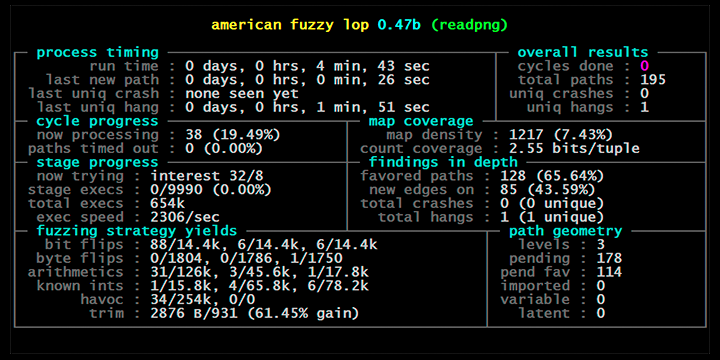
\includegraphics[width=\textwidth]{Chapter2/afl_screen.png}
    \centering
    \caption{AFL status screen}
    \label{fig:status_screen}
\end{figure} 

\begin{enumerate}
    \item \textbf{Process timing}: This section tells about how long the fuzzing process is running.
    
    \item \textbf{Overall results}: A simplified information about the progress of AFL in finding paths, hangs, and crashes. 

    \item \textbf{Cycle progress}: As mentioned before, AFL takes one input and repeats mutating it for a while. This section shows the information about the current cycle that the fuzzer is working with.

    \item \textbf{Map coverage}: The AFL's documentation explains the information in this section as: \say{The section provides some trivia about the coverage observed by the instrumentation embedded in the target binary. The first line in the box tells you how many branches we have already hit, in proportion to how much the bitmap can hold. The number on the left describes the current input; the one on the right is the entire input corpus's value. The other line deals with the variability in tuple hit counts seen in the binary. In essence, if every taken branch is always taken a fixed number of times for all the inputs we have tried, this will read "1.00". As we manage to trigger other hit counts for every branch, the needle will start to move toward "8.00" (every bit in the 8-bit map hit) but will probably never reach that extreme. 
    
    Together, the values can help compare the coverage of several different fuzzing jobs that rely on the same instrumented binary.}

    \item \textbf{Stage progress}: The information about the current mutation stage is briefly provided here. This regards to \texttt{fuzz\_one()} function in which the new fuzzed inputs are being generated through mutation stages.

    \item \textbf{Findings in depth}: The number of crashes and hangs and any other findings are presented in this section.

    \item \textbf{Fuzzing strategy yields}: To illustrate more stats about the strategies used since the beginning of fuzzing. For the comparison of those strategies, AFL keeps track of how many paths it has explored, in proportion to the number of executions attempted.

    \item \textbf{Path geometry}: The information about the inputs and their depths, which says how many generations of different paths were produced in the process. The depth of an input referes to which generation the input belongs to. Considering the first input seeds as depth 0, the generated population from these inputs increase the depth by one. This shows how far the fuzzing has progressed.
\end{enumerate}

\subsection{AFL fuzzing chain}

\begin{figure}[!t]
    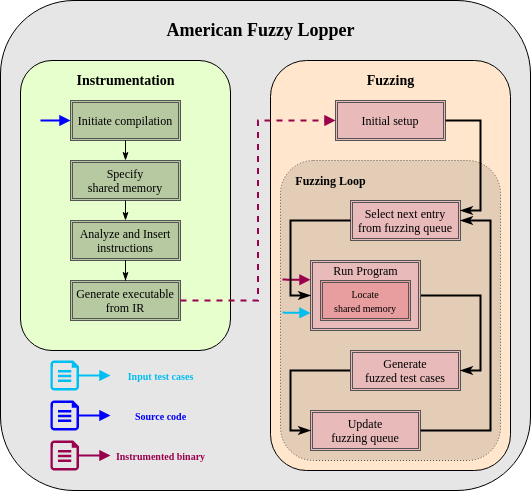
\includegraphics[width=\textwidth]{Chapter2/AFL-proc.png}
    \centering
    \caption{An overview of the whole fuzzing procedure of AFL}
    \label{fig:afl-proc}
\end{figure}

Figure \ref{fig:afl-proc} illustrates the procedure of fuzzing, from static intrumentation to fuzz testing the target and outputing results. To start the procedure, AFL instrumentates the program and configures the target binary for fuzz testing stage. To perform the instrumentation, AFL calls its own compiler, which applies the instrumentation when it's process is finished [Listing \ref{lst:sample_inst}]: 

\begin{lstlisting}[language=bash,style=CommandStyle,label={lst:sample_inst},caption=Instrument $sample\_vul$.c]
    afl-clang sample.c -o sample_inst
\end{lstlisting}

The result file, \texttt{sample\_inst}, is an executable which contains shared memory for later analysis in fuzzing. Now AFL can start testing the program for probable vulnerabilities. The test requires the input and output directories, as well as the command for executing the program [Listing \ref{lst:fuzz_inst}]. The fuzzing continues until recieving a halt signal (For instance, by pressing \textit{Ctrl+C}). 

\begin{lstlisting}[language=bash,style=CommandStyle,label={lst:fuzz_inst},caption=Execute AFL]
  # afl-fuzz -i <in_dir> -o <out_dir> [options] -- /path/to/fuzzed/app [params]
  afl-fuzz -i in_dir -o out_dir -- ./sample_inst
\end{lstlisting}